\documentclass[12pt,a4paper,oneside]{article}
\usepackage{geometry}
\geometry{a4paper,scale=0.7}
\usepackage{graphics}
\usepackage{indentfirst}
\usepackage{amsmath}
\usepackage{algorithm}
\usepackage{algorithmic}
\usepackage{bm}
\usepackage{setspace}
\usepackage{graphicx}
\usepackage{float}
\usepackage{CJKutf8}
\usepackage{hyperref}
\usepackage{color}
\usepackage{listings}

\definecolor{dkgreen}{rgb}{0,0.6,0}
\definecolor{gray}{rgb}{0.5,0.5,0.5}
\definecolor{mauve}{rgb}{0.58,0,0.82}

\author{Ruichen Wang}
\title{Tensorflow Serving基础与应用}
\begin{document}
\begin{CJK*}{UTF8}{gbsn}

\maketitle
\begin{abstract}
Tensorflow serving 基础与应用,介绍tensorflow serving基本概念,应用示例和性能评估。
\end{abstract}

\section{介绍}
TF Serving是TensorFlow官方提供的一套用于模型服务的框架,目标就是实现在线,低延迟的预测服务。它的突出优点是:和TensorFlow无缝链接,可以将训练好的机器学习模型部署到线上,支持多模型多版本同时serving,支持HTTP/gRPC作为接口接受外部调用。TensorFlow Serving支持模型热更新与自动模型版本管理,对扩展性的支持和性能都非常好。目前业内有很多公司已经采用此技术来提供服务,也是阿里云提供的深度学习预测服务的唯一选择。


\begin{figure}[H]
\centering
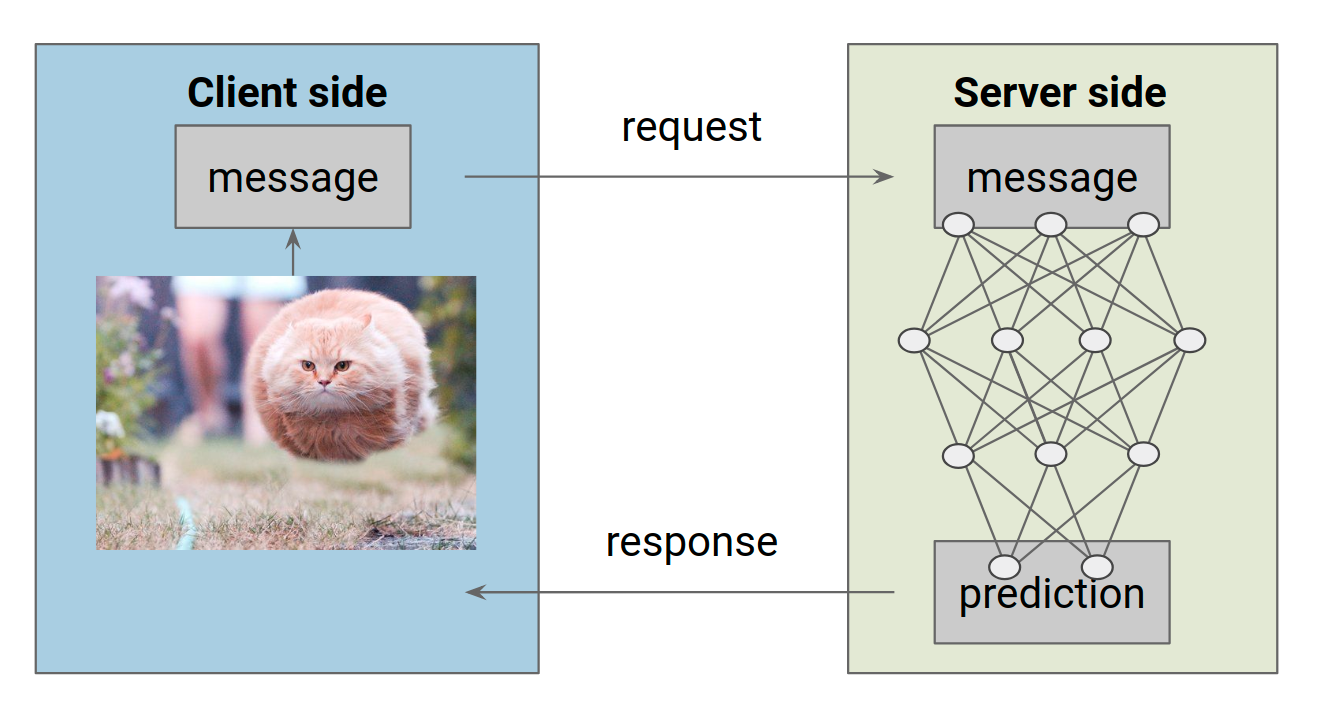
\includegraphics[width=4in,height=2in]{tfserving}
\caption{Tensorflow Serving}
\end{figure}

\paragraph{features:}
\begin{itemize}
\item Can serve multiple models, or multiple versions of the same model simultaneously
\item Exposes both gRPC as well as HTTP inference endpoints
\item Allows deployment of new model versions without changing any client code
\item Supports canarying new versions and A/B testing experimental models
\item Adds minimal latency to inference time due to efficient, low-overhead implementation
\item Features a scheduler that groups individual inference requests into batches for joint execution on GPU, with configurable latency controls
\item  Supports many servables: Tensorflow models, embeddings, vocabularies, feature transformations and even non-Tensorflow-based machine learning models
\end{itemize}

在实际场景中,算法的整个流程应该包括数据准备和预处理,模型训练,预测服务三大块。Tensorflow Serving主要应用于模型的预测服务中。针对我们的信息流推荐实际业务,采用deepfm模型,完全可以实现毫秒级的响应。批量预测1000个case也只需要0.3ms左右的时间。


\begin{figure}[H]
\centering
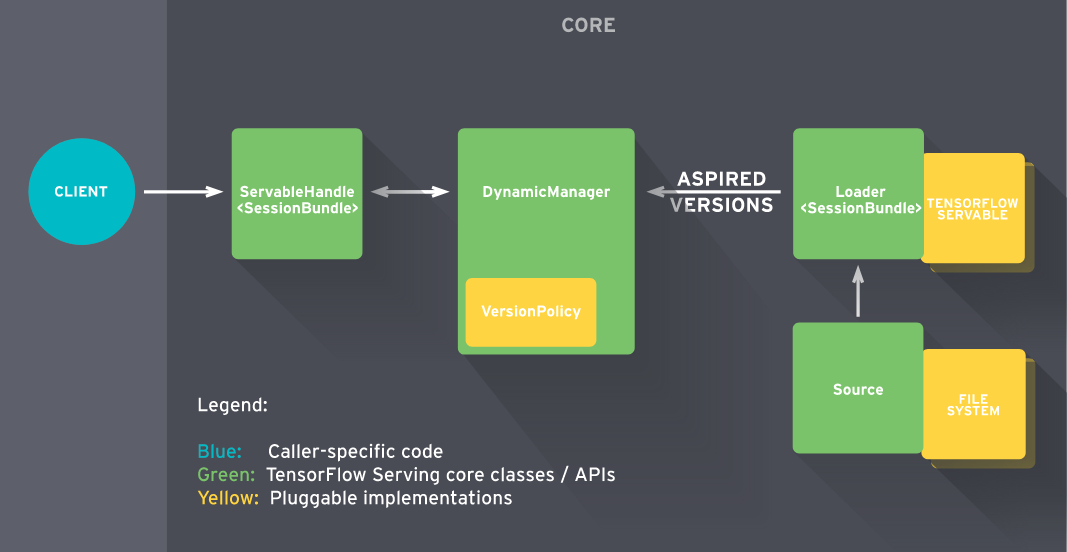
\includegraphics[width=6in,height=3in]{lifeofservable}
\caption{life of a servable}
\end{figure}
Source组件为特定的模型版本创建一个Loader,其中包含用作serving的所有元数据。 同时通知Manager最新的版本号。由manager来决定是否需要重新加载之前版本或者最新版本。客户端请求时可以默认使用最新版本,也可以指定访问某一固定版本。

一些Extension组件介绍:
\begin{itemize}
\item Version Policy
- 主要提供两种版本控制协议 Availability Preserving Policy 和 Resource Preserving Policy
\item Source 
\item Loader
\item Batcher
- 用于控制batch size, 线程数,batch队列,超时时间等
\end{itemize}


\section{生成模型}
Tensorflow提供了多种保存模型的方法。

\begin{lstlisting}
tf.saved_model.simple_save (keras)
estimator.export.build_parsing_serving_input_receiver_fn
estimator.export.build_raw_serving_input_receiver_fn
\end{lstlisting}

最简单的可以使用simple save方法,以key-value的格式,指定模型输入和输出。一般结合keras model一起使用。这也是tensorflow 2.0以后比较的方法。另外使用estimator.export提供的两个接口,更方便结合feature column导出。在目前tensorflow1.14适用性更广一些。

\begin{figure}[H]
\centering
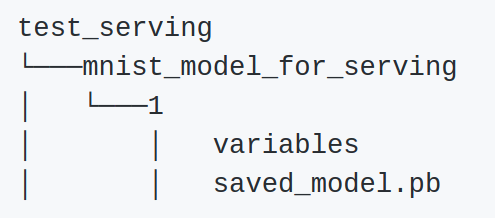
\includegraphics[width=3in,height=1.2in]{modelpath}
\caption{saved model path}
\end{figure}

\begin{figure}[H]
\centering
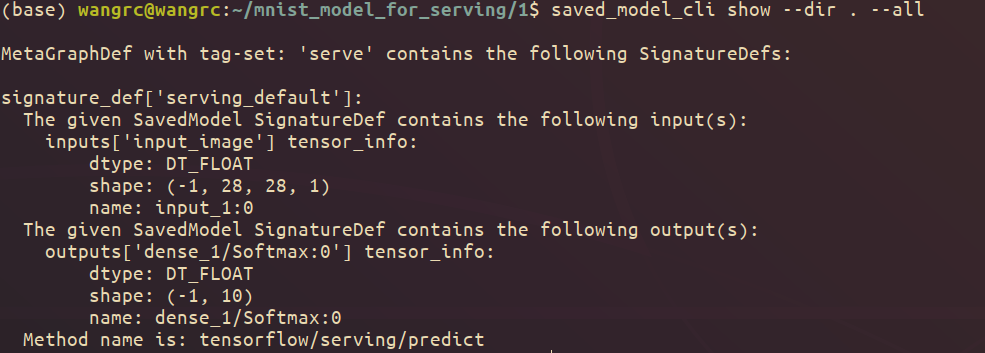
\includegraphics[width=6in,height=2in]{savedmodelcli}
\caption{savedmodelcli}
\end{figure}
模型文件保存后,会生成对应版本号的文件夹,在同一个模型目录下,tesorflow serving会默认自动加载版本号最新的模型文件,tensorflow提供了bash命令来查看保存的模型接口和输出结果,方便client调用。

保存模型的时候,可以定义Classify, Regress或者Predict API。以predict为例,在保存模型时指定predict的signature key, 调用时只要在客户端请求指定的method name接口就可以了。

\begin{itemize}
\item Regress : 1 input tensor, 1 output tensor.
\item Classify : 1 input tensor, output classes \& scores.
\item Predict : arbitray many input and output tensors.
\end{itemize}


\begin{figure}[H]
\centering
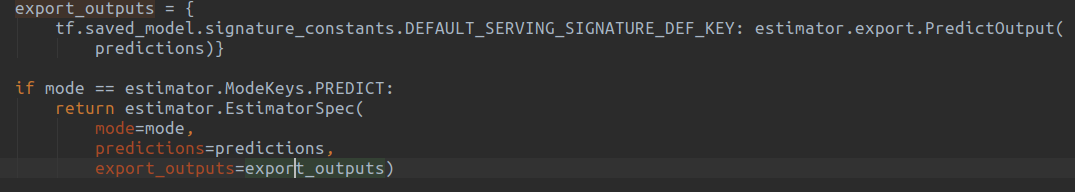
\includegraphics[width=6in,height=1.2in]{predictapi}
\caption{predict api}
\end{figure}

\section{提供服务}
有了模型文件,我们就可以部署我们的模型服务了。主要有以下三种方案:
\begin{itemize}
\item tensorflow model server + 单节点
\item docker + 单节点
\item docker + k8s + 集群部署
\end{itemize}
在测试阶段,可以采用第一种或者第二种,可以方便调试与测试模型性能等指标。如果真正部署至生产环境,就需要依托k8s的的平台,提供服务注册与发现,负载均衡,链路监控,网关路由等一系列微服务功能。

\paragraph{•} 如果是ubuntu系统,可以方便的使用apt安装 tensorlfow model server。其他情况,推荐采用docker方法。

参考链接 \url{https://www.tensorflow.org/tfx/serving/setup}。

\paragraph{•} 使用docker比较简单,只需要拉取tensorlfow serving镜像,然后docker run一下就行了。推荐直接采用docker的方法来测试模型服务。这也是最方便的使用gpu版本的serving的方法。在官方docker镜像中,默认使用8500作为grpc调用接口,8501作为REST调用接口。可以通过-p命令映射到宿主其他端口上。
\begin{lstlisting}
docker pull tensorflow/serving
\end{lstlisting}

\begin{figure}[H]
\centering
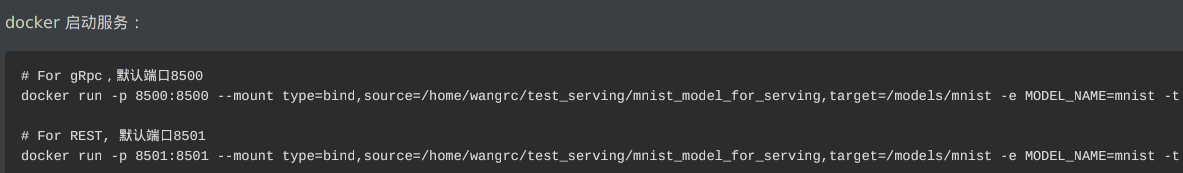
\includegraphics[width=6in,height=1in]{dockerstart}
\caption{docker service start}
\end{figure}

\paragraph{•} 在生产环境,模型服务一般需要在集群上部署,需要支持较大的QPS。可以采用k8s来编排部署。可以自己指定副本数量与计算资源。在副本出现问题的时候k8s会重新拉起,同时保证分配计算资源。
\begin{figure}[H]
\centering
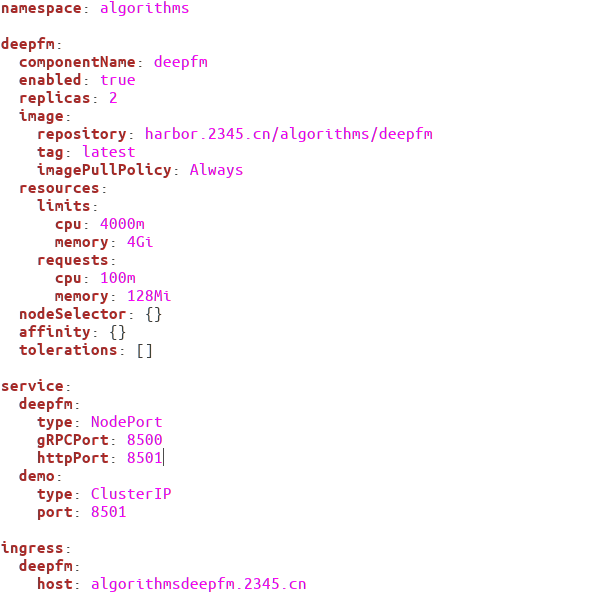
\includegraphics[width=4in,height=4in]{k8s}
\caption{k8s yaml}
\end{figure}

\section{客户端调用}
在目前的tensorflow提供了查看模型服务状态的方法,同时也为客户端提供了gPRC和REST两种调用模式。

\paragraph{REST}
使用REST方法时,数据使用json字符串格式传输,使用utf-8编码。值得注意的是,如果输入的数据是二进制格式的,需要将字符串转化成Base64的格式。另外,一般我们常用的float类型的特征经常会出现inf或者nan。 默认的json也不能识别此类数据。需要使用json parser进行转换。


\begin{figure}[H]
\centering
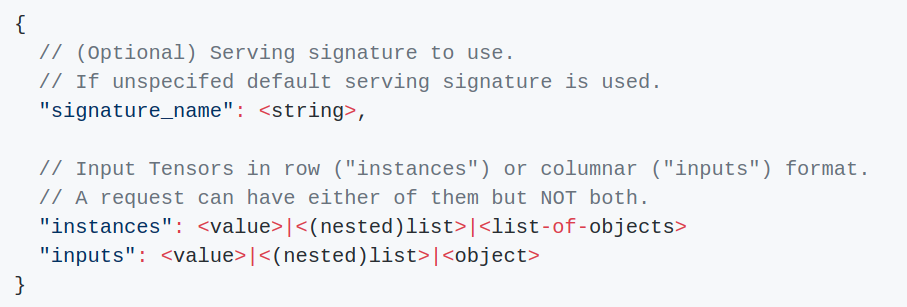
\includegraphics[width=6in,height=2.1in]{requestformat}
\caption{request format}
\end{figure} 

\begin{figure}[H]
\centering
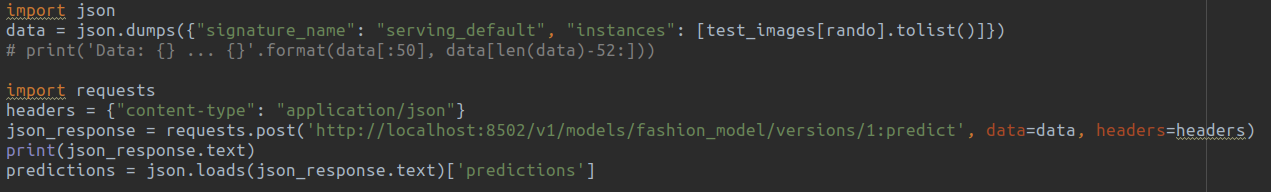
\includegraphics[width=6in,height=1.0in]{restrequest}
\caption{rest request demo}
\end{figure}

\paragraph{gPRC}
在实际应用中,如果特征维度比较高,或者是直接传输图像数据,这时候数据量一般比较大,进行json转化会比较耗时,拼接成的字符串也会较大,传输时间往往会是瓶颈。这时候就可以考虑使用grpc调用。一般情况下,同样的数据,使用grpc实际传输字节只有json的一半,配合serialize example格式,模型预测速度也有3倍左右的提高。

在模型serving的时候,可以同时对外提供grpc和rest接口,客户端可以根据应用需要选择对应的接口。

\begin{itemize}
\item REST (serialized once)
\begin{itemize}
\item Inference rate: 7,680 img/sec
\item Network: 620 MB
\end{itemize}
\item gPRC (serialized once)
\begin{itemize}
\item Inference rate: 25,961 img/sec
\item Network: 320 MB
\end{itemize}
\end{itemize}

\begin{figure}[H]
\centering
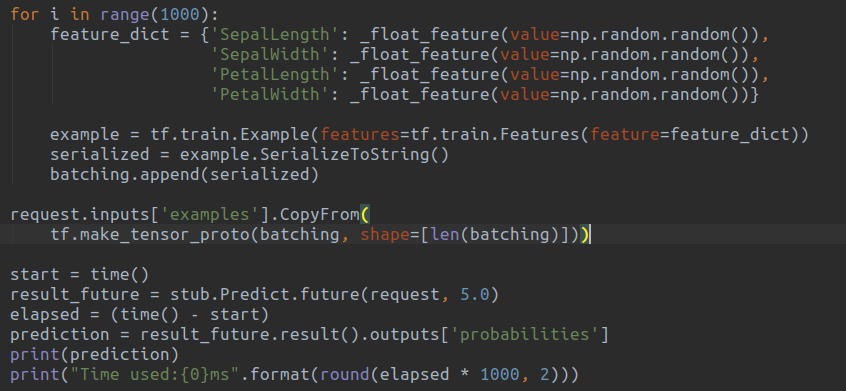
\includegraphics[width=6in,height=3.0in]{grpcclient}
\caption{grpc client demo}
\end{figure}


\section{版本切换warmup}
tf serving在模型版本切换的时候,初始的几个case响应时间会明显高于正常水平。这种情况主要是因为tensorflow 运行时采用 lazily initialization的方式。 tensorflow可以自定义warm up request。保存一个用于warmup的tfrecords。 这样每次模型加载的时候,会先调用tfrecords里的样本先做几次预测,初始化相关组件。

\section{demo示例}

\section{问题}


\end{CJK*}
\end{document}

























